\section{Příklad 1}
% Jako parametr zadejte skupinu (A-H)
\prvniZadani{F}

\begin{center}
    \begin{LARGE}
        Řešení metodou postupného zjednodušování
    \end{LARGE}
\end{center}

% Krok 1
\begin{figure}[h]
    \centering
    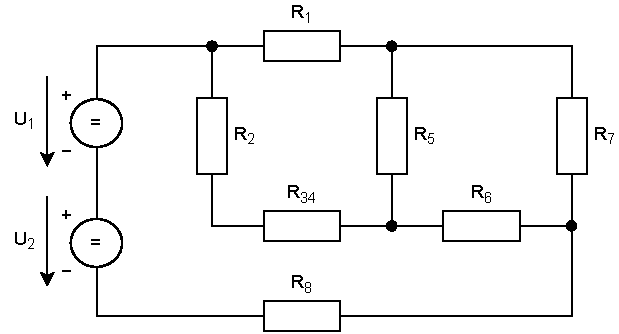
\includegraphics[scale=0.8,keepaspectratio]{fig/Pr1_krok1.pdf}
    \caption{Zjednodušení $R_3$ a $R_4$ (paralelní zapojení)}
    \label{pic:Pr1_krok1}
\end{figure}

\begin{center}
    \begin{gather*}
        R_{34} = \frac{R_3 \times R_4}{R_3+R_4} = \frac{550 \times 250}{550+250} = 171,875 \: \Omega
    \end{gather*}
\end{center}

\newpage

% Krok 2
\begin{figure}[h]
    \centering
    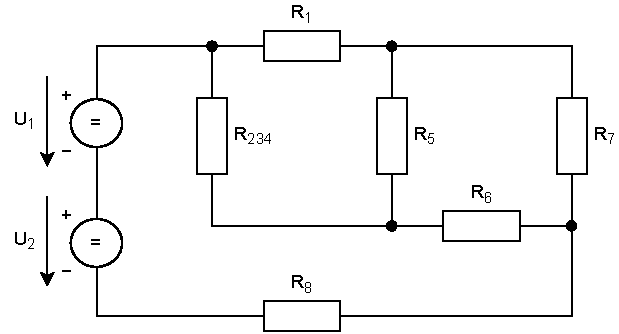
\includegraphics[scale=0.8,keepaspectratio]{fig/Pr1_krok2.pdf}
    \caption{Zjednodušení $R_2$ a $R_{34}$ (sériové zapojení)}
    \label{pic:Pr1_krok2}
\end{figure}

\begin{center}
    \begin{gather*}
        R_{234} = R_2 + R_{34} = 500 + 171,875 = 671,875 \: \Omega
    \end{gather*}
\end{center}

% Krok 3
\begin{figure}[h]
    \centering
    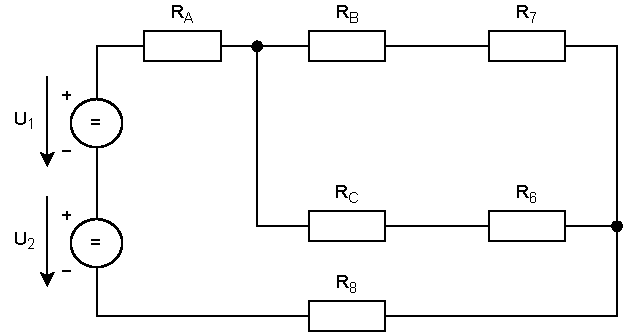
\includegraphics[scale=0.8,keepaspectratio]{fig/Pr1_krok3.pdf}
    \caption{Trojúhelník -> hvězda}
    \label{pic:Pr1_krok3}
\end{figure}

\begin{center}
    \begin{gather*}
        R_A = \frac{R_1 \times R_{234}}{R_1+R_{234}+R_5} = \frac{550 \times 671,875}{510+671,875+300} = 231,2315 \: \Omega \\[6pt]
        R_B = \frac{R_1 \times R_5}{R_1+R_{234}+R_5} = \frac{550 \times 300}{510+671,875+300} = 103,2476 \: \Omega \\[6pt]
        R_C = \frac{R_{234} \times R_5}{R_1+R_{234}+R_5} = \frac{671,875 \times 300}{510+671,875+300} = 136,0186 \: \Omega
    \end{gather*}
\end{center}

\newpage

% Krok 4
\begin{figure}[h]
    \centering
    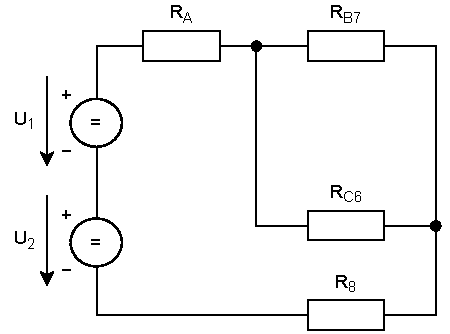
\includegraphics[scale=0.8,keepaspectratio]{fig/Pr1_krok4.pdf}
    \caption{Zjednodušení $R_B$ a $R_7$, $R_C$ a $R_6$ (sériové zapojení)}
    \label{pic:Pr1_krok4}
\end{figure}

\begin{center}
    \begin{gather*}
        R_{B7} = R_B + R_7 = 103,2476 + 330 = 433,2476 \: \Omega \\
        R_{C6} = R_C + R_6 = 136,0186 + 800 = 936,0186 \: \Omega
    \end{gather*}
\end{center}

% Krok 5
\begin{figure}[h]
    \centering
    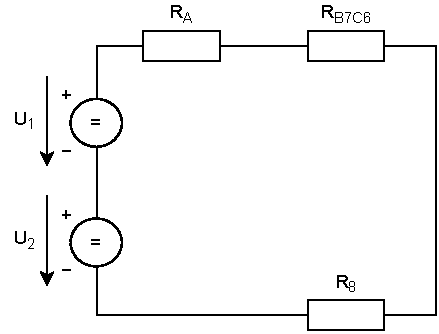
\includegraphics[scale=0.8,keepaspectratio]{fig/Pr1_krok5.pdf}
    \caption{Zjednodušení $R_{B7}$ a $R_{C6}$ (paralelní zapojení)}
    \label{pic:Pr1_krok5}
\end{figure}

\begin{center}
    \begin{gather*}
        R_{B7C6} = \frac{R_{B7} \times R_{C6}}{R_{B7}+R_{C6}} = \frac{433,2476 \times 936,0186}{433,2476+936,0186} = 296,1643 \: \Omega
    \end{gather*}
\end{center}

% Krok 6
\begin{figure}[h]
    \centering
    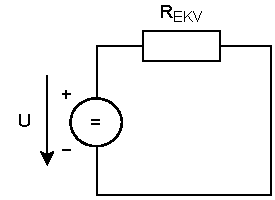
\includegraphics[scale=0.8,keepaspectratio]{fig/Pr1_krok6.pdf}
    \caption{Zjednodušení $R_A$, $R_{B7C6}$, $R_8$ a $U_1$, $U_2$ (sériové zapojení)}
    \label{pic:Pr1_krok6}
\end{figure}

\begin{center}
    \begin{gather*}
        R_{EKV} = R_A + R_{B7C6} + R_8 = 231,2315 + 296,1643 + 250 = 777,3958 \: \Omega \\
        U = U_1 + U_2 = 125 + 65 = 190 \: V \\\\
    \end{gather*}
\end{center}

% Krok7
\begin{itemize}
    \item Spočítáme proud I (Ohmův zákon)
\end{itemize}

\begin{center}
    \begin{gather*}
        I = \frac{U}{R_{EKV}} = \frac{190}{777,3958} = 0,2444 \: A \\
    \end{gather*}
\end{center}

% Krok 8
\begin{itemize}
    \item Spočítáme $U_{R_8}$, $U_{R_A}$ (Ohmův zákon) a $U_{R_{B7C6}}$ (sériové zapojení)
\end{itemize}

\begin{center}
    \begin{gather*}
        U_{R_8} = I * R_8 = 0,2444 \times 250 = 61,1 \: V \\
        U_{R_A} = I * R_A = 0,2444 \times 231,2315 = 56,513 V \: \\
        U_{R_{B7C6}} = U - U_{R_8} - U_{R_A} = 190 - 61,1 - 56,513 = 72,387 \: V \\
    \end{gather*}
\end{center}

% Krok 9
\begin{itemize}
    \item $I_{R_{C6}}$ se rovná $I_{R_6}$ (sériové zapojení), tedy můžeme spočítat $I_{R_6}$ a $U_{R_6}$ (Ohmův zákon)
\end{itemize}

\begin{center}
    \begin{gather*}
        I_{R_{C6}} = I_{R_6} = \frac{U_{R_{C6}}}{R_{C_6}} = \frac{72,387}{936,0186} = 0,0773 \: A \\[6pt]
        U_{R_6} = I_{R_6} \times R_6 = \frac{72,387}{936,0186} \times 800 = 61,868 \: V
    \end{gather*}
\end{center}